\usetikzlibrary{arrows.meta,shapes.multipart,patterns}

\tikzset{
    stackBox/.style={very thick},
    onStack/.style={thick},
    frameOne/.style={fill=blue!15},
    frameTwo/.style={fill=red!15},
    markLine/.style={blue!50!black},
    markLineB/.style={red!90!black},
    hiLine/.style={red!90!black},
}

\begin{frame}{malloc/new guard pages}
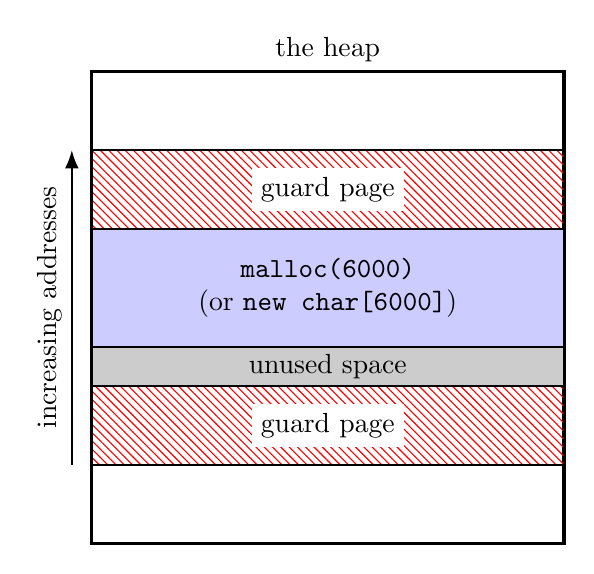
\begin{tikzpicture}
    \draw[thick,-Latex] (-0.25,-5) -- (-0.25, -1) node [midway, above, sloped] {increasing addresses};
    \node[anchor=south] at (3, 0) {the heap};
    \draw[stackBox] (0, 0) rectangle (6, -6);
    \draw[onStack,fill=blue!20] (0, -2) rectangle (6, -3.5)
        node[midway,align=center] {\texttt{malloc(6000)} \\ (or \texttt{new char[6000]}) };
    \draw[onStack,pattern=north west lines,pattern color=red] (0, -1) rectangle (6, -2)
        node[midway,fill=white] {guard page};
    \draw[onStack,pattern=north west lines,pattern color=red] (0, -4) rectangle (6, -5)
        node[midway,fill=white] {guard page};
    \draw[onStack,fill=black!20] (0, -3.5) rectangle (6, -4)
        node[midway] {unused space};
\end{tikzpicture}
\end{frame}

\begin{frame}{guard pages}
    \begin{itemize}
    \item deliberate holes
    \item accessing --- segfualt
    \item call to OS to allocate (not very fast)
    \item likely to `waste' memory
        \begin{itemize}
        \item guard around object? minimum 4KB object
        \end{itemize}
    \end{itemize}
\end{frame}

\begin{frame}{guard pages for malloc/new}
    \begin{itemize}
    \item can implement malloc/new by placing guard pages around allocations
        \begin{itemize}
        \item commonly done by real malloc/new's for \myemph{large allocations}
        \end{itemize}
    \item problem: minimum actual allocation 4KB
    \item problem: substantially slower
    \item example: ``Electric Fence'' allocator for Linux (early 1990s)
    \end{itemize}
\end{frame}


\begin{frame}[fragile]{guard pages and arrays/structs}
\begin{Verbatim}
struct foo {
    char buffer[1000];
    /* can't really put guard page here */
    int *ptr;
};
\end{Verbatim}
\begin{itemize}
\item C compiler expects buffer and ptr to be adjacent
\item can't add guard page without changing all code that accesses \texttt{struct foo}
\item similar poblem with separating elements of arrays
\end{itemize}
\end{frame}
